\documentclass[11pt,a4paper]{article}
\usepackage[margin=25mm]{geometry}
\usepackage{graphicx,booktabs,siunitx,amsmath,microtype,caption}
\usepackage{float}
\usepackage[table]{xcolor}
\usepackage[hidelinks]{hyperref}
\usepackage{fancyhdr}
\definecolor{ink}{HTML}{14171C}
\definecolor{ink2}{HTML}{565C66}
\definecolor{rule2}{HTML}{D3D8E0}
\definecolor{accent}{HTML}{2A78D6}
\definecolor{warnbg}{HTML}{FDF6E7}
\definecolor{alertbg}{HTML}{FDF0EF}
\definecolor{rowbg}{HTML}{F4F5F7}
\captionsetup{font=small,labelfont=bf,labelsep=period,width=.95\textwidth}
\sisetup{detect-all,group-minimum-digits=4}
\pagestyle{fancy}\fancyhf{}
\fancyhead[L]{\footnotesize\color{ink2}TRIGA Mark I --- Cross-Code Reference Calculation}
\fancyhead[R]{\footnotesize\color{ink2}\thepage}
\renewcommand{\headrulewidth}{0.4pt}

\newcommand{\keff}{\ensuremath{k_{\mathrm{eff}}}}
\newcommand{\kinf}{\ensuremath{k_{\infty}}}
\newcommand{\pcm}{\,pcm}

\newsavebox{\calloutbox}
\newenvironment{callout}[2][warnbg]
 {\edef\calloutcolor{#1}\def\callouttitle{#2}%
  \begin{lrbox}{\calloutbox}%
  \begin{minipage}{\dimexpr\textwidth-2\fboxsep\relax}%
  \vspace{1mm}\par\textbf{\footnotesize\MakeUppercase{\callouttitle}}\par\vspace{1mm}\small}
 {\vspace{1mm}\end{minipage}\end{lrbox}%
  \par\vspace{2mm}\noindent\colorbox{\calloutcolor}{\usebox{\calloutbox}}\par\vspace{2mm}}

\begin{document}
\begin{titlepage}
\vspace*{15mm}
{\footnotesize\color{ink2}\textsc{Cross-code reference calculation}\hfill September 2026, revised October 2026}\par
\vspace{3mm}\hrule height 1pt \vspace{8mm}
{\Huge\bfseries TRIGA Mark I\par}
\vspace{3mm}
{\LARGE Independent neutronic and thermal-hydraulic\\[2mm] reference calculations in
GeN-Foam and Cardinal\par}
\vspace{10mm}
{\large A code-to-code study of a 250\,kW pool-type research reactor, comparing a
deterministic OpenFOAM multiphysics solution (GeN-Foam) against a stochastic
Monte Carlo reference (Cardinal).\par}
\vspace{8mm}
{\large Kavya Wadhwa\par}
\vspace{10mm}
{\small\begin{tabular}{@{}ll@{}}
\toprule
\textbf{GeN-Foam} & 2-group diffusion, finite volume\\
\textbf{Cardinal} & OpenMC / MOOSE / NekRS --- continuous-energy Monte Carlo\\
\midrule
Nuclear data & ENDF/B-VIII.0 (VII.1 for the Cardinal coupled run)\\
Repository & \texttt{github.com/kavyawadhwa134/triga-crosscode-verification}\\
Blind comparison & Cardinal frozen by git tag before GeN-Foam results were read\\
\bottomrule
\end{tabular}}
\vfill
\begin{callout}[alertbg]{Status of this document}
This report presents \textbf{verification and a cross-code comparison}. It is
\textbf{not a validation report}. No experimental data was used in either calculation, and
agreement between two codes is not a substitute for measurement. Section~\ref{sec:status}
states the status of each verification level explicitly.
\end{callout}
\end{titlepage}

\tableofcontents
\newpage

%======================================================================
\section{Problem definition}
\subsection{Objective}
Two separate calculations of the same TRIGA Mark I configuration were performed using
fundamentally different numerical methods, with the goal of establishing a cross-code
reference. Only the scientific problem definition was shared between the two models. The
comparison was made blind: the Cardinal results were frozen under the git tag
\texttt{pcm-independent-v1} before any GeN-Foam result was read, which is verifiable from the
repository history.

The TRIGA Mark I is a pool-type research reactor whose defining characteristic is
uranium--zirconium hydride fuel. Hydrogen bound in the ZrH lattice produces a large, prompt,
negative fuel temperature coefficient, which is the physical basis of the reactor's inherent
safety. Reproducing that feedback correctly is the principal physics requirement on any
TRIGA model.

\subsection{Specification}
\begin{table}[H]\centering\small
\caption{Shared problem specification. Values marked \emph{assumed} were not given and are
documented modelling choices.}
\begin{tabular}{@{}llp{62mm}@{}}
\toprule
\textbf{Parameter} & \textbf{Value} & \textbf{Basis}\\
\midrule
Fuel outer radius & \SI{1.815}{\centi\meter} & specification\\
Clad outer radius & \SI{1.866}{\centi\meter} & specification\\
Lattice pitch (square) & \SI{4.235}{\centi\meter} & specification\\
Active height & \SI{60.0}{\centi\meter} & specification\\
Core & \SI{0.495}{\meter} $\times$ \SI{0.60}{\meter} & single zone, vacuum; shape not stated\\
\midrule
Fuel U--ZrH$_{1.65}$ & \SI{6.0}{\gram\per\cubic\centi\meter} &
  U-235 1.7, U-238 6.8, Zr 89.862, H-1 1.638\,wt\%\\
Clad SS304 & \SI{8.00}{\gram\per\cubic\centi\meter} & density \emph{assumed}\\
Coolant & \SI{1.0}{\gram\per\cubic\centi\meter} & H$_2$O, unborated\\
\midrule
Thermal power & \SI{250}{\kilo\watt} & specification\\
Coolant inlet & \SI{293}{\kelvin}, \SI{0.2}{\meter\per\second} & specification\\
Pressure & \SI{0.1}{\mega\pascal} & \emph{assumed} --- open pool\\
Energy groups & 2, cutoff \SI{0.625}{\electronvolt} & specification\\
\bottomrule
\end{tabular}
\end{table}

The core extent ``0.495 $\times$ 0.60\,m'' admits more than one reading. Cardinal models it as
a 3-D cylinder of diameter \SI{0.495}{\meter}; GeN-Foam models it as a 2-D slab
\SI{0.495}{\meter} wide and \SI{0.60}{\meter} tall, infinite in the third direction. This
difference in interpretation turns out to dominate the core eigenvalue comparison
(Section~\ref{sec:comp}).

There is no fuel--clad gap: the specification gives two radii, so the clad inner radius
equals the fuel outer radius. Thermal scattering $S(\alpha,\beta)$ data for
\texttt{c\_H\_in\_ZrH} and \texttt{c\_Zr\_in\_ZrH} is mandatory; without it the
bound-hydrogen physics that defines a TRIGA is absent.

\subsection{The two approaches}
\begin{table}[H]\centering\small
\caption{The two calculations solve different equations. This distinction governs the
interpretation of every comparison in Section~\ref{sec:comp}.}
\begin{tabular}{@{}lll@{}}
\toprule
 & \textbf{GeN-Foam} & \textbf{Cardinal}\\
\midrule
Neutron transport & Deterministic, 2-group diffusion & Monte Carlo, continuous energy\\
Energy treatment & 2 groups, \SI{0.625}{\electronvolt} cutoff & Continuous, full spectrum\\
Core geometry & 2-D slab, homogenised & 3-D cylinder, heterogeneous (+ homogenised)\\
Thermal--fluid & Finite volume, OpenFOAM & Spectral element, implicit LES\\
Fuel conduction & Sub-scale pin model & 3-D finite element (MOOSE)\\
Transient & Yes ($+0.5\,\$$ insertion) & Out of scope\\
Solution error & Discretisation, not quantified & Statistical, quantified ($\pm$\,pcm)\\
\bottomrule
\end{tabular}
\end{table}

\subsection{Acceptance criterion}
The project sets \textbf{500\pcm{} on $k$} as the flag for a material difference.
Section~\ref{sec:comp} applies this criterion only between
methodologically comparable quantities.

\newpage
%======================================================================
\section{Results: GeN-Foam}
\subsection{Solver acceptance}
Prior to the TRIGA calculation, GeN-Foam was verified against its own reference cases.

\begin{table}[H]\centering\small
\caption{GeN-Foam solver acceptance (\texttt{validation\_step2.csv}).}
\begin{tabular}{@{}llrrl@{}}
\toprule
\textbf{Case} & \textbf{Quantity} & \textbf{Simulated} & \textbf{Expected} & \textbf{Status}\\
\midrule
3D SmallESFR & \keff & 0.936873 & 0.936827 & PASS ($4.9\times10^{-5}$)\\
2D point kinetics & steady state & --- & --- & PASS\\
2D point kinetics & transient, no driveline & --- & --- & PASS\\
2D point kinetics & transient, driveline & --- & --- & PASS\\
2D point kinetics & transient, boron & --- & --- & PASS\\
\bottomrule
\end{tabular}
\end{table}

\subsection{Lattice constants}
GeN-Foam condensed its own two-group constants from an OpenMC pin-cell calculation
(70 batches, 20 inactive, 8000 particles per batch), giving
$\kinf = 1.38810 \pm 0.00123$.

\begin{table}[H]\centering\small
\caption{GeN-Foam two-group lattice constants (\texttt{validation\_step5.csv}).}
\begin{tabular}{@{}lrr@{}}
\toprule
\textbf{Quantity} & \textbf{Fast} & \textbf{Thermal}\\
\midrule
Removal (\si{\per\meter}) & 4.77341 & 8.49190\\
$\nu\Sigma_f$ (\si{\per\meter}) & 0.379899 & 12.5219\\
Diffusion coefficient (\si{\meter}) & 0.00749023 & 0.00158363\\
$\chi$ & 1.0 & 0.0\\
Inverse velocity (\si{\second\per\meter}) & $6.62997\times10^{-6}$ & $3.31676\times10^{-4}$\\
\midrule
$S_{1\rightarrow1}$ & 39.7524 & \\
$S_{1\rightarrow2}$ & 4.22693 & \\
$S_{2\rightarrow1}$ & 0.023426 & \\
$S_{2\rightarrow2}$ & & 201.932\\
\bottomrule
\end{tabular}
\end{table}

\begin{callout}{Consistency of the group constants}
Solving the two-group constants above analytically for an infinite medium gives
$\kinf = 1.38873$, against the Monte Carlo lattice value of $1.38810$ --- a difference of
$+33$\pcm{}. The condensation therefore preserves the lattice eigenvalue, and the constants
are not a significant error source in the core comparison. (The same file also lists
\texttt{genfoam\_smoke\_keff} $=1.331$; this is a diffusion solution on a separate 2-D channel
test geometry with leakage, not on the pin cell, so it is not a method benchmark.)
\end{callout}

\subsection{Steady state}
The core is modelled as a bare homogenised \textbf{2-D slab}, \SI{0.495}{\meter} wide and
\SI{0.60}{\meter} tall, one cell thick with \texttt{empty} front and back patches (so infinite in
the third direction), on a $20\times24$ mesh with zero flux imposed on the boundary.

\begin{table}[H]\centering\small
\caption{GeN-Foam steady-state results (\texttt{validation\_step6.csv}).}
\begin{tabular}{@{}llp{52mm}@{}}
\toprule
\textbf{Quantity} & \textbf{Value} & \textbf{Note}\\
\midrule
\keff & 1.240544 & eigenvalue diffusion, bare homogenised 2-D slab, zero-flux boundary\\
Power & \SI{250}{\kilo\watt} & target\\
Max coolant temperature & \SI{306.47}{\kelvin} & fluid $T$\\
Max average fuel temperature & \SI{594.2}{\kelvin} & sub-scale pin average; well below the \SI{1023}{\kelvin} limit\\
Power peaking (max/avg) & 2.45 & cosine--cosine shape; analytic slab value $\pi^2/4=2.47$\\
\bottomrule
\end{tabular}
\end{table}

\begin{figure}[H]\centering
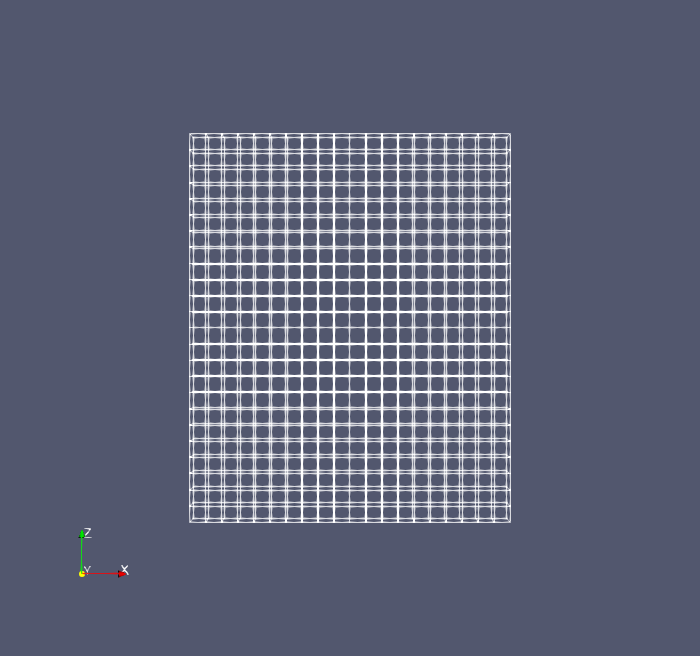
\includegraphics[width=.48\textwidth]{fig/genfoam_mesh.png}\hfill
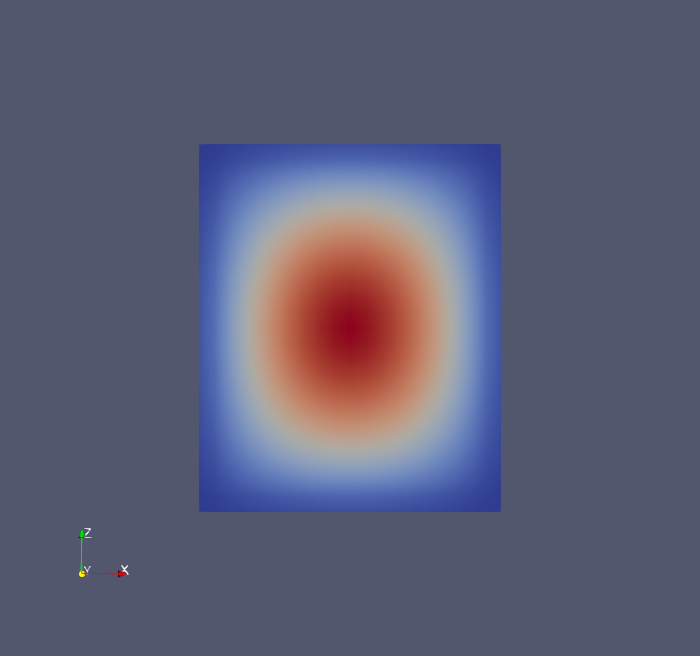
\includegraphics[width=.48\textwidth]{fig/genfoam_steady_power.png}
\caption{GeN-Foam computational mesh (left) and steady-state power density (right).}
\end{figure}

\begin{figure}[H]\centering
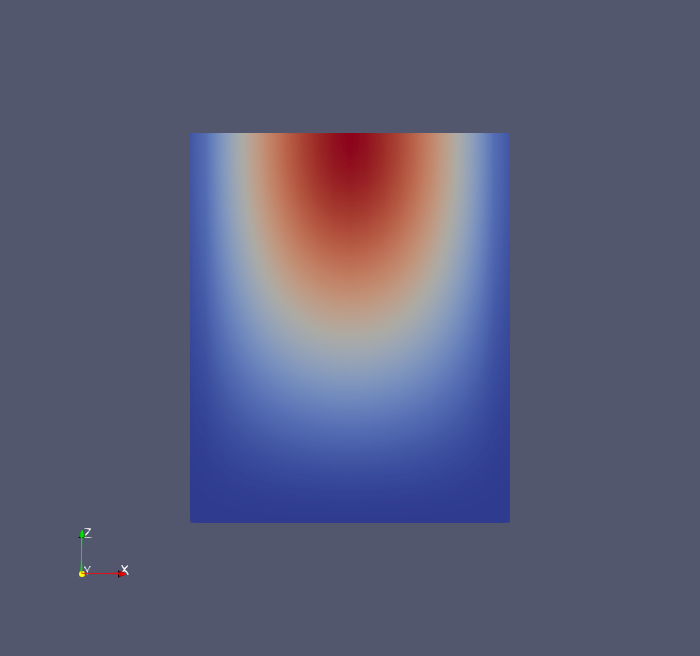
\includegraphics[width=.60\textwidth]{fig/genfoam_steady_T.png}
\caption{GeN-Foam steady-state temperature field. The maximum lies in the upper portion of the
core, consistent with coolant heating as it rises through the channel.}
\end{figure}

\subsection{Reactivity insertion transient}
A $+0.5\,\$$ ramp ($0.00325\,\Delta k/k$) was inserted between $t=100$ and
$t=\SI{100.5}{\second}$.

\begin{figure}[H]\centering
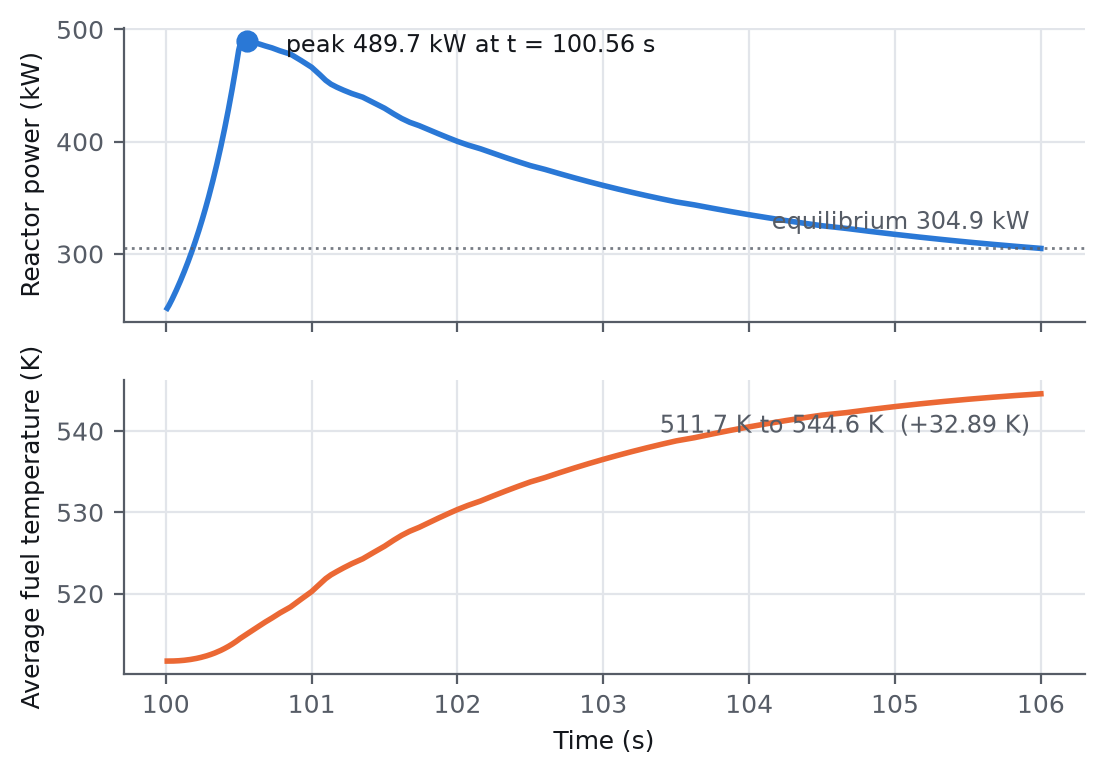
\includegraphics[width=\textwidth]{fig/genfoam_transient.png}
\caption{GeN-Foam transient response. Power peaks at \SI{489.7}{\kilo\watt} and settles to a
Doppler-limited equilibrium of \SI{304.9}{\kilo\watt}; average fuel temperature rises
\SI{32.89}{\kelvin}.}
\end{figure}

\begin{table}[H]\centering\small
\caption{GeN-Foam transient summary.}
\begin{tabular}{@{}lrl@{}}
\toprule
\textbf{Quantity} & \textbf{Value} & \textbf{Note}\\
\midrule
Peak power & \SI{489723}{\watt} & at $t=\SI{100.56}{\second}$\\
Final power & \SI{304884}{\watt} & Doppler-limited equilibrium\\
Final average fuel $T$ & \SI{544.59}{\kelvin} & at $t=\SI{106}{\second}$\\
Net reactivity & $-3.87$\pcm & external $+325$ vs Doppler $-328.9$\\
\bottomrule
\end{tabular}
\end{table}

\begin{callout}{Feedback coefficient is an input, not a result}
The stated Doppler feedback of $-328.9$\pcm{} accompanies a fuel temperature rise from
511.70 to \SI{544.59}{\kelvin}, a span of \SI{32.89}{\kelvin}:
\[
\frac{-328.9\pcm}{\SI{32.89}{\kelvin}} = -10.000\ \mathrm{pcm/K}.
\]
The result is \emph{exactly} $-10.000$ because the coefficient is a constant model input:
\texttt{feedbackCoeffTFuel} $=-1.0\times10^{-4}\,\mathrm{K}^{-1}$ in the point-kinetics
\texttt{nuclearData} of the transient case, taken from a published TRIGA prompt fuel temperature
coefficient (University of Texas TRIGA overview) rather than computed for this model. The transient uses
U-235 Keepin six-group delayed-neutron data and a prompt generation time of
\SI{43}{\micro\second}. Section~\ref{sec:comp} compares the coefficient against Cardinal's
computed value.
\end{callout}

\newpage
%======================================================================
\section{Results: Cardinal / OpenMC / MOOSE / NekRS}
\subsection{Method}
Continuous-energy Monte Carlo neutronics (OpenMC) is coupled to finite-element heat
conduction (MOOSE) through Cardinal by Picard iteration: cell-averaged fission power is
transferred to the solid, and cell temperatures are returned to the neutronics. The coolant
is treated separately by spectral-element large-eddy simulation (NekRS).

Because the available hardware could not support a full-core coupled model, the coupled
calculation uses a \textbf{single-pin unit cell}. All coupled temperatures therefore
describe an \emph{average} pin.

\subsection{Neutronics}
\begin{table}[H]\centering\small
\caption{Cardinal eigenvalue results, ENDF/B-VIII.0, continuous-energy Monte Carlo.}
\begin{tabular}{@{}llrr@{}}
\toprule
\textbf{Quantity} & \textbf{Model} & \textbf{Value} & \textbf{Uncertainty}\\
\midrule
\kinf & 2-D unit cell, reflective & 1.384207 & $\pm\,21$\pcm\\
\keff & 3-D bare core, heterogeneous & 1.102059 & $\pm\,26$\pcm\\
\keff & 3-D bare core, homogenised & 1.145259 & $\pm\,74$\pcm\\
Leakage fraction & bare core & 0.20149 & $\pm\,0.00012$\\
Power peaking (max/avg) & 120 pins & 2.2544 & ---\\
Peak power density & bare core & \SI{6.595}{\watt\per\cubic\centi\meter} & ---\\
\bottomrule
\end{tabular}
\end{table}

The homogenised variant was computed specifically to separate geometry treatment from
solution method in the comparison of Section~\ref{sec:comp}. Its sensitivity to the
$S(\alpha,\beta)$ choice is itself notable: 1.145259 (H in H$_2$O), 1.132505 (H in ZrH) and
1.136651 (none) span 1275\pcm, more than twice the acceptance criterion.

\subsection{Fuel temperature coefficient}
The defining TRIGA parameter was computed from first principles by sweeping fuel temperature
with the moderator held at \SI{293}{\kelvin}, isolating fuel feedback.

The sweep was performed on the \textbf{reflective unit cell}, so the eigenvalue it returns is
$\kinf$ by construction: with reflective boundaries on all six faces there is no leakage, and
no $\keff$ exists for that model. This isolates the fuel feedback mechanism itself --- the
change in the neutron balance within the lattice --- from the leakage response of a finite
core. Section~\ref{sec:leak} shows why that distinction is quantitatively important here.

\begin{figure}[H]\centering
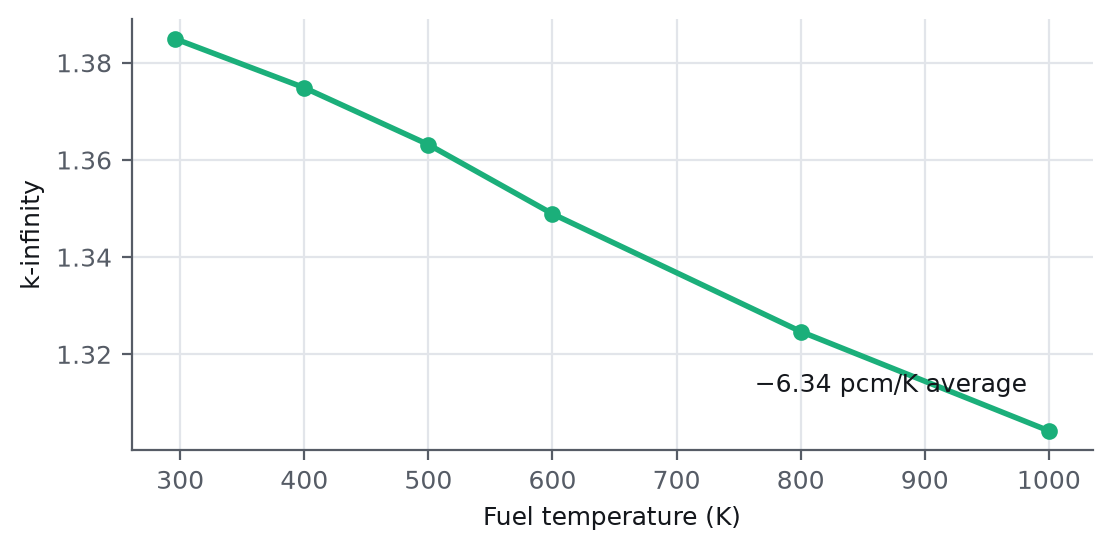
\includegraphics[width=.82\textwidth]{fig/fig4_tempcoeff.png}
\caption{Cardinal fuel temperature coefficient. $\kinf$ falls from 1.384926 at
\SI{296}{\kelvin} to 1.304249 at \SI{1000}{\kelvin}.}
\end{figure}

\begin{table}[H]\centering\small
\caption{Cardinal local fuel temperature coefficient by interval ($\pm1\sigma$, Monte Carlo
statistics).}
\begin{tabular}{@{}lr@{}}
\toprule
\textbf{Band} & \textbf{Coefficient}\\
\midrule
296--\SI{400}{\kelvin} & $-5.08\pm0.43$\,pcm/K\\
400--\SI{500}{\kelvin} & $-6.24\pm0.46$\,pcm/K\\
\rowcolor{rowbg}500--\SI{600}{\kelvin} & $\mathbf{-7.76\pm0.47}$\,\textbf{pcm/K}\\
600--\SI{800}{\kelvin} & $-6.78\pm0.23$\,pcm/K\\
800--\SI{1000}{\kelvin} & $-5.92\pm0.24$\,pcm/K\\
\midrule
296--\SI{1000}{\kelvin} average & $-6.34$\,pcm/K\\
\bottomrule
\end{tabular}
\end{table}

The coefficient is large, negative, and becomes \emph{more} negative as the fuel heats from room
temperature. Both
features identify this as hydride physics rather than U-238 Doppler: a UO$_2$ LWR pin gives
roughly $-2$ to $-3$\,pcm/K and its magnitude does not grow in this way. The highlighted band
is the one in which the GeN-Foam transient operates.


\subsection{Leakage feedback: the coefficient on a finite core}\label{sec:leak}
The coefficient above is an infinite-lattice quantity. In a finite core the eigenvalue is
$\keff = \kinf \, P_{\mathrm{NL}}$, where $P_{\mathrm{NL}}$ is the non-leakage probability, so
the measurable reactivity coefficient carries a second term:
\[
\frac{1}{\keff}\frac{\partial \keff}{\partial T_f}
= \underbrace{\frac{1}{\kinf}\frac{\partial \kinf}{\partial T_f}}_{\text{lattice feedback}}
+ \underbrace{\frac{1}{P_{\mathrm{NL}}}\frac{\partial P_{\mathrm{NL}}}{\partial T_f}}_{\text{leakage feedback}}.
\]
The leakage term is not negligible in this problem, because the bare core leaks
\textbf{20.1\%} of its neutrons. Physically, heating the hydride up-scatters thermal neutrons
off the $\sim$\SI{0.14}{\electronvolt} ZrH oscillator, hardening the in-fuel spectrum. A harder
spectrum has a longer migration length, so a larger fraction escapes a finite core:
$P_{\mathrm{NL}}$ falls with fuel temperature and the leakage term is \emph{negative},
reinforcing the lattice feedback.

The sweep was therefore repeated on the bare heterogeneous core with vacuum boundaries.

\begin{table}[H]\centering\small
\caption{Fuel temperature coefficient with and without leakage. The leakage term contributes
20--36\% of the total and grows with temperature.}
\begin{tabular}{@{}lrrrr@{}}
\toprule
\textbf{Band (K)} & \textbf{$\kinf$ (unit cell)} & \textbf{$\keff$ (bare core)} &
\textbf{Leakage term} & \textbf{Share}\\
\midrule
296--400 & $-5.08$ & $-6.31\pm0.73$ & $-1.23$ & 20\%\\
400--500 & $-6.24$ & $-9.12\pm0.78$ & $-2.88$ & 32\%\\
\rowcolor{rowbg}
500--600 & $-7.76$ & $\mathbf{-10.79\pm0.82}$ & $-3.04$ & 28\%\\
600--800 & $-6.78$ & $-10.61\pm0.42$ & $-3.83$ & 36\%\\
800--1000 & $-5.92$ & $-9.10\pm0.44$ & $-3.18$ & 35\%\\
\bottomrule
\end{tabular}
\end{table}

\begin{figure}[H]\centering
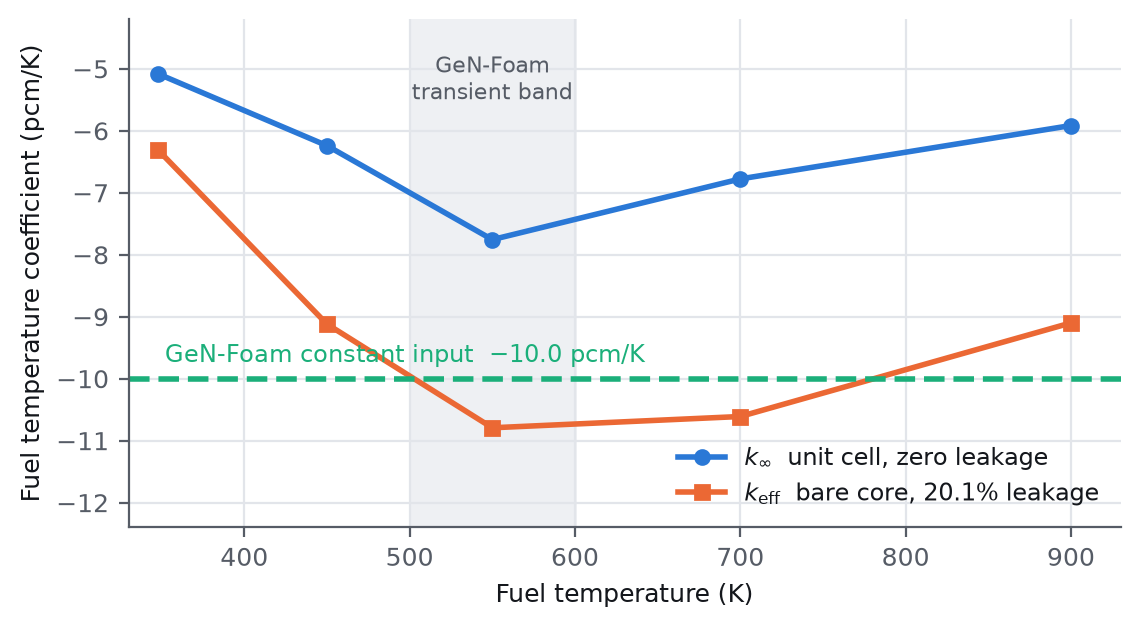
\includegraphics[width=.86\textwidth]{fig/fig8_leakage_feedback.png}
\caption{Fuel temperature coefficient computed with and without leakage. All values in
pcm/K, plotted at band midpoints.}
\end{figure}

Both curves suggest a maximum magnitude between about 500 and \SI{800}{\kelvin}, consistent
with the up-scattering effect saturating once the thermal population has been pushed clear of
the ZrH oscillator energy; the turnover is resolved at roughly the $2\sigma$ level only.
\textbf{The $\keff$-based coefficient is the one that governs a core transient}, and it is
25--55\% more negative than the lattice value across the whole range.

\subsection{Coupled neutronics--conduction}
\begin{figure}[H]\centering
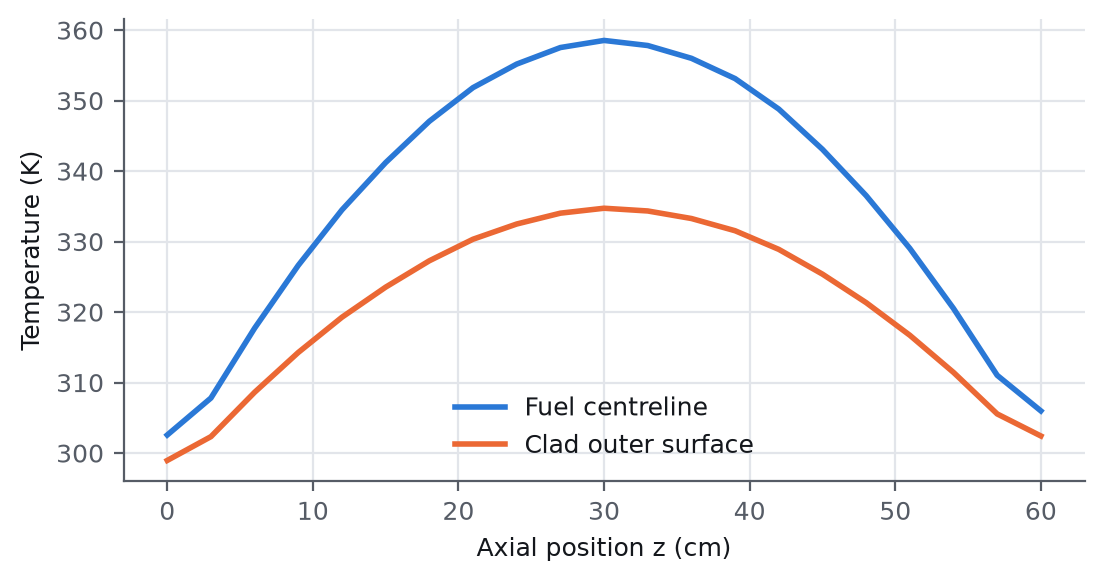
\includegraphics[width=.49\textwidth]{fig/fig1_axial.png}\hfill
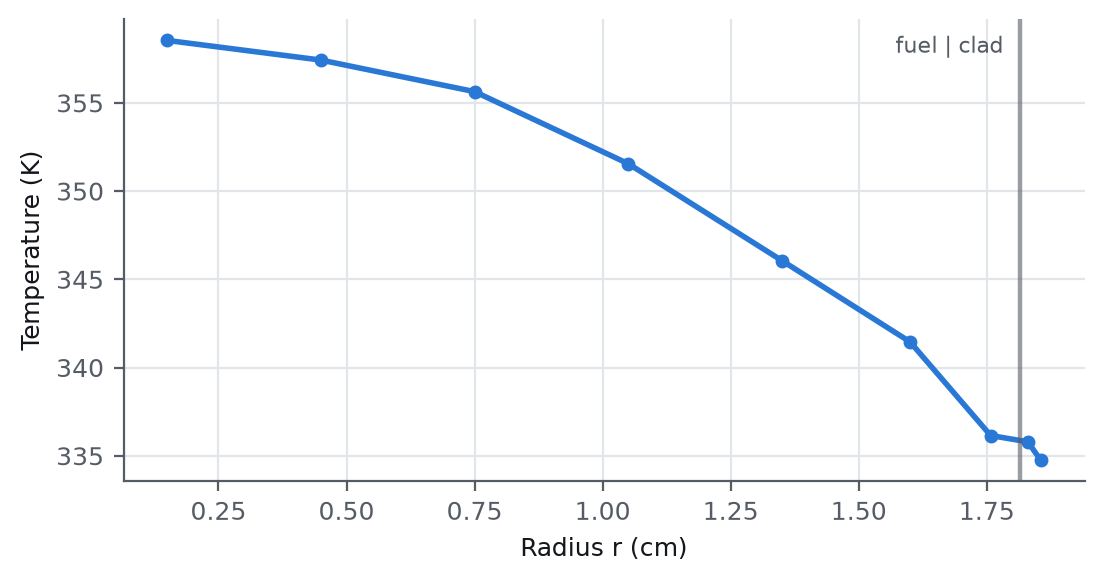
\includegraphics[width=.49\textwidth]{fig/fig2_radial.png}
\caption{Cardinal coupled temperature solution. Left: axial profile, slightly top-skewed
(\SI{305.98}{\kelvin} outlet against \SI{302.56}{\kelvin} inlet) because the coolant heats as
it rises. Right: radial profile at mid-plane; temperature is continuous across the
fuel--clad interface at \SI{1.815}{\centi\meter}, confirming the stitched contact.}
\end{figure}

\begin{table}[H]\centering\small
\caption{Cardinal coupled results and temperature drop budget.}
\begin{tabular}{@{}lrrr@{}}
\toprule
\textbf{Quantity} & \textbf{Value} & \textbf{Analytic} & \textbf{Share}\\
\midrule
Peak fuel temperature & \SI{359.0}{\kelvin} & \SI{362.8}{\kelvin} & ---\\
Peak clad temperature & \SI{336.2}{\kelvin} & --- & ---\\
Power integral & \SI{2083.33}{\watt} & \SI{2083.33}{\watt} & exact\\
\midrule
Film drop (clad $\rightarrow$ coolant) & \SI{40.3}{\kelvin} & \SI{42.4}{\kelvin} & 63\%\\
Fuel conduction drop & \SI{22.4}{\kelvin} & \SI{24.1}{\kelvin} & 35\%\\
Clad conduction drop & \SI{1.07}{\kelvin} & \SI{1.5}{\kelvin} & 2\%\\
\bottomrule
\end{tabular}
\end{table}

Agreement with the analytic cylindrical-conduction solution is within 1.1\%; the residual is
explained by the true axial power shape being flatter than the cosine the hand calculation
assumes. The film drop dominates and is the least certain term --- it derives from a
Dittus--Boelter correlation at $\mathrm{Re}=4755$, which is transitional and below the range
where that correlation is reliable.

\begin{figure}[H]\centering
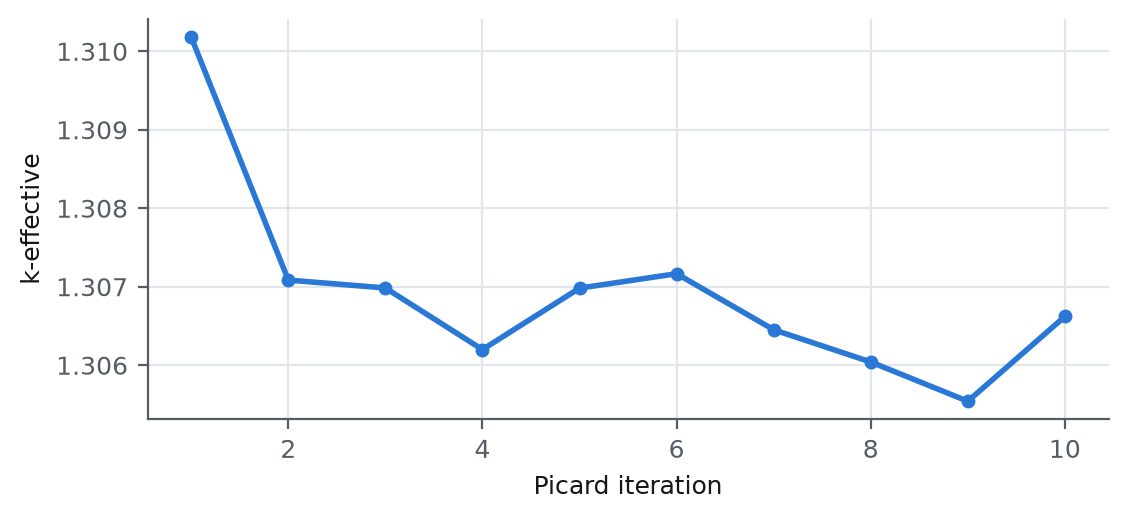
\includegraphics[width=.78\textwidth]{fig/fig3_picard.png}
\caption{Cardinal Picard convergence. $\keff$ settles within Monte Carlo noise after the first
temperature feedback; average fuel temperature is stable to \SI{e-8}{\kelvin}.}
\end{figure}

\subsection{Thermal-hydraulics}
An implicit large-eddy simulation of the coolant subchannel was run at $\mathrm{Re}=4755$,
polynomial order 7, 2880 spectral elements, on an NVIDIA GTX 1080~Ti. The run completed
20\,000 steps but covered only \textbf{1.17 flow-through times}. A conservation check after the
run also found that only 59\% of the clad surface carried the heated-wall boundary tag in the
committed mesh; the mesh generator has been corrected but the mesh has not yet been
regenerated. The CFD is therefore a \textbf{diagnostic of the GPU workflow}, and none of its
temperatures is used in a result or comparison.

\begin{figure}[H]\centering
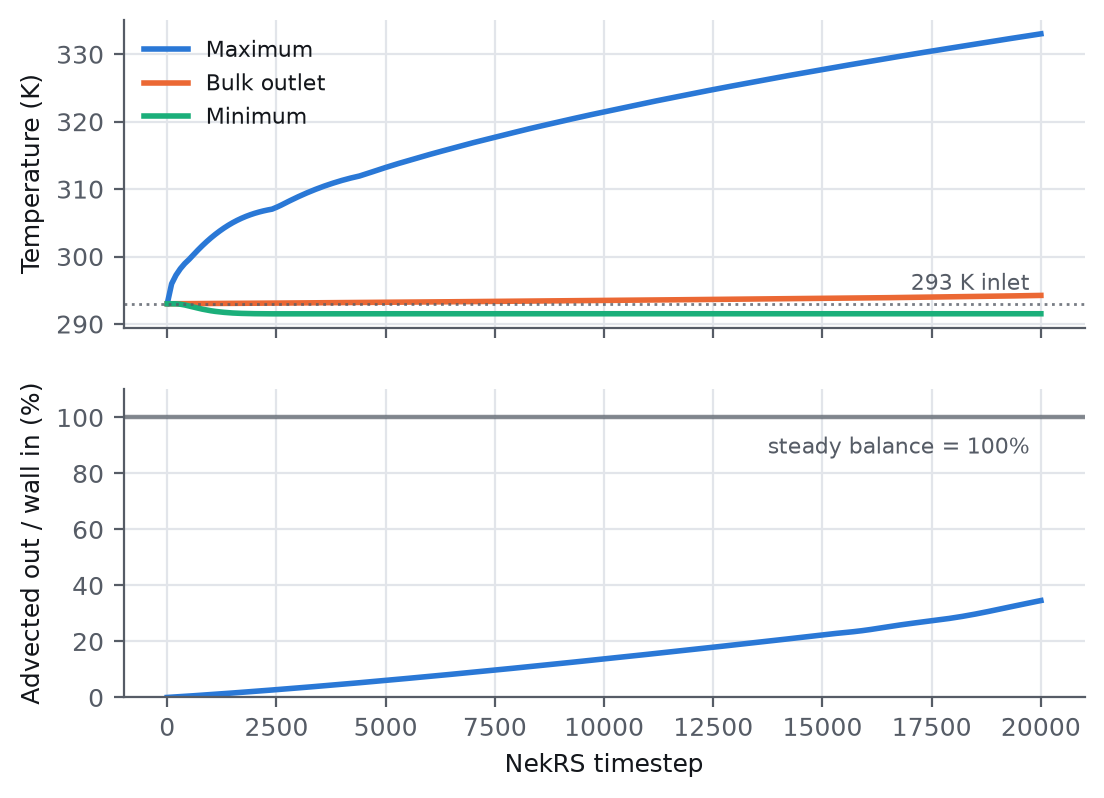
\includegraphics[width=.85\textwidth]{fig/fig7_nekrs.png}
\caption{Cardinal NekRS evolution. Upper: coolant temperatures, all still rising at the final
step, with the minimum below the \SI{293}{\kelvin} inlet throughout. Lower: energy closure
reaches only 34.6\% of the steady balance.}
\end{figure}

\begin{table}[H]\centering\small
\caption{Cardinal thermal-hydraulic state at 20\,000 steps.}
\begin{tabular}{@{}lrrl@{}}
\toprule
\textbf{Quantity} & \textbf{Value} & \textbf{Steady target} & \textbf{Status}\\
\midrule
Bulk outlet temperature & \SI{294.24}{\kelvin} & \SI{296.57}{\kelvin} & not physical\\
Maximum temperature & \SI{333.03}{\kelvin} & --- & still rising\\
Minimum temperature & \SI{291.52}{\kelvin} & $\geq$ \SI{293}{\kelvin} & unphysical\\
Advected heat / wall heat & 34.6\% & 100\% & not closed\\
Mass-flow imbalance & 0.122\% & $\rightarrow 0$ & converged\\
\bottomrule
\end{tabular}
\end{table}

\begin{callout}[alertbg]{The Cardinal coolant CFD is a diagnostic, not a result}
The flow field has converged --- mass imbalance is flat at 0.122\% from step 1400 onward ---
but only 34.6\% of the wall heat leaves the domain, so 65.4\% is still accumulating.
Together with the incomplete heated-wall tagging, this means \textbf{the coolant temperatures
above are not physical results.} Reaching
approximately five flow-throughs would require about 85\,700 steps and \SI{5.1}{\hour} of
GPU time.

A second defect is recorded rather than smoothed over: the minimum temperature lies below
the inlet in a domain whose only thermal boundary conditions are a \SI{293}{\kelvin} inlet
and a heated wall. With no heat sink this cannot be physical. It is an undershoot from the
high-pass filter stabilisation and it does not decay.
\end{callout}


\subsection{Nuclear data sensitivity}
The specification requires ENDF/B-VIII.0. The execution environment for the coupled run
carried ENDF/B-VII.1, so the identical coupled model was run on both libraries and the
difference recorded as a measured offset rather than left as an unknown.

\begin{table}[H]\centering\small
\caption{Library sensitivity of the coupled Cardinal model.}
\begin{tabular}{@{}llrrr@{}}
\toprule
\textbf{Library} & \textbf{Platform} & \textbf{\keff} & \textbf{Max fuel $T$} & \textbf{Tally error}\\
\midrule
ENDF/B-VIII.0 & macOS arm64, 5k particles & 1.30561 & \SI{358.64}{\kelvin} & 2.06\%\\
ENDF/B-VII.1 & Ubuntu x86, 20k particles & 1.30656 & \SI{358.90}{\kelvin} & 0.82\%\\
\midrule
\rowcolor{rowbg}
Difference & VII.1 $-$ VIII.0 & $+73$\pcm & $+\SI{0.25}{\kelvin}$ & ---\\
\bottomrule
\end{tabular}
\end{table}

\SI{73}{}\pcm{} is small relative to the acceptance criterion and within combined counting
statistics. The same comparison also demonstrates \textbf{cross-platform reproducibility}:
average fuel temperature agrees to \SI{7e-4}{\kelvin} between macOS~arm64 and Ubuntu~x86,
across different libraries and different particle budgets.

\newpage
%======================================================================
\section{Comparison}\label{sec:comp}
\subsection{Overview}
\begin{table}[H]\centering\small
\caption{Case-by-case comparison. Only cases marked \emph{yes} support a direct numerical
difference; the acceptance criterion applies to those alone.}
\begin{tabular}{@{}clrrrl@{}}
\toprule
\textbf{\#} & \textbf{Case} & \textbf{GeN-Foam} & \textbf{Cardinal} & \textbf{Difference} & \textbf{Comparable}\\
\midrule
\rowcolor{rowbg}
1 & \kinf, unit cell & $1.388100$ & $1.384207$ & $-280$\pcm & yes\\
2 & \keff, as modelled & $1.240544$ & $1.102059$ & $\Delta\rho=+10129$\pcm & no$^c$\\
3 & \keff, same cylinder & $1.140929$$^a$ & $1.145259$ & $\Delta\rho=-331$\pcm & yes\\
4 & Group constants, \kinf & $1.38873$$^a$ & --- & $+33$\pcm$^b$ & internal\\
5 & Fuel temp.\ coefficient & $-10.000$ & $-10.79\pm0.82$ & $+7\%$ & yes\\
6 & Power peaking & $2.45$ & $2.2544$ & $-8.0\%$ & no$^c$\\
7 & Max fuel temperature & \SI{594.2}{\kelvin} & \SI{359.0}{\kelvin} & $-\SI{235}{\kelvin}$ & no\\
8 & Max coolant temperature & \SI{306.5}{\kelvin} & diagnostic only & --- & no\\
9 & Total power & \SI{250}{\kilo\watt} & \SI{250}{\kilo\watt} & $0$ & yes\\
10 & Transient peak power & \SI{489.7}{\kilo\watt} & not run & --- & no\\
11 & Two-group MGXS & full set & not generated & --- & no\\
12 & Solver acceptance & PASS & not recorded & --- & no\\
\bottomrule
\end{tabular}

\vspace{1mm}\footnotesize $^a$ GeN-Foam two-group constants solved analytically
(\texttt{keff\_decomposition.py}). $^b$ Against GeN-Foam's own OpenMC lattice, 1.38810.
$^c$ Different core geometry: 2-D slab vs 3-D cylinder.
\end{table}

\subsection{Case 1 --- the directly comparable quantity}
Both sides solved the same 2-D reflective pin cell with OpenMC continuous-energy Monte Carlo
and ENDF/B-VIII.0. This is the only case in which the two calculations solve the same
equations on the same geometry.

\begin{figure}[H]\centering
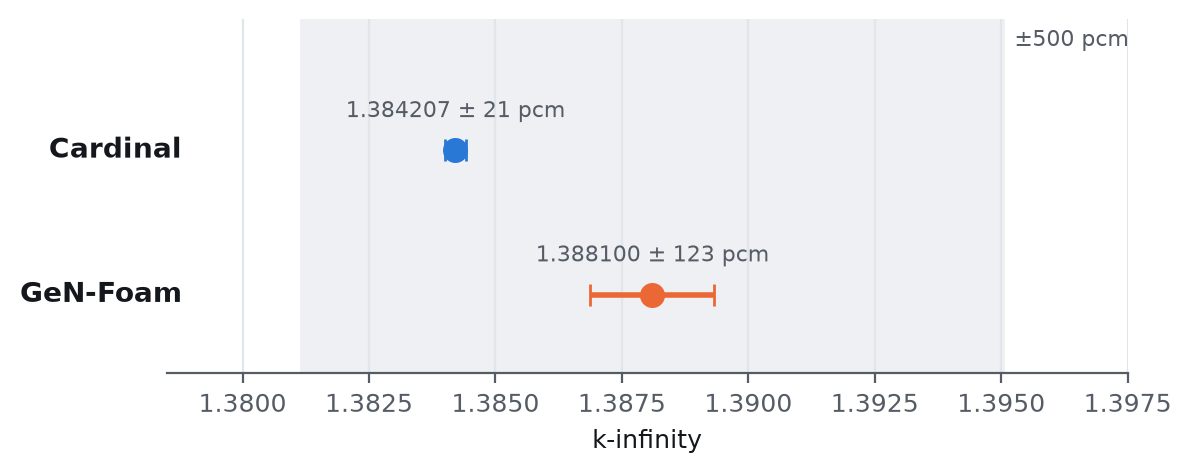
\includegraphics[width=.82\textwidth]{fig/fig5_kinf.png}
\caption{$\kinf$ comparison. Bars are $\pm 1\sigma$ counting statistics; the shaded band is
the 500\pcm{} acceptance criterion centred on GeN-Foam.}
\end{figure}

The difference is $\mathbf{-280}$\,\textbf{pcm} at $3.1\sigma$ --- statistically resolved but
comfortably inside the acceptance criterion. Cardinal's uncertainty is approximately six times
tighter, reflecting a 25-fold larger particle budget.

\emph{Interpretation.} Two separate implementations of the same specification, in the same
code, agree. A small part of the residual is expected from a documented input difference: the
SS304 cladding was defined at \SI{8.00}{\gram\per\cubic\centi\meter} in Cardinal and
\SI{7.9}{\gram\per\cubic\centi\meter} with slightly different trace elements in the GeN-Foam
lattice. This is the strongest evidence in the study that the shared problem definition
was interpreted consistently on both sides.

\subsection{Cases 2--4 --- the \keff{} difference is mostly geometry}
The two core eigenvalues differ by $\Delta\rho=+10\,129$\pcm{}, but the two models differ in more
than solution method. GeN-Foam's mesh is a 2-D slab (\SI{49.5}{\centi\meter} $\times$
\SI{60}{\centi\meter}, \texttt{empty} front and back, zero flux on the boundary); Cardinal's
core is a 3-D cylinder of diameter \SI{49.5}{\centi\meter} and height \SI{60}{\centi\meter}. The
slab has no leakage in its third direction, so its geometric buckling is only 56\% of the
cylinder's.

To separate the effects, GeN-Foam's own two-group constants were solved analytically for a
bare homogeneous core in each geometry, and the difference was decomposed into additive
reactivity steps ($\rho=1-1/k$). The analysis is reproducible with
\texttt{keff\_decomposition.py} in \texttt{results/comparison/}.

\begin{figure}[H]\centering
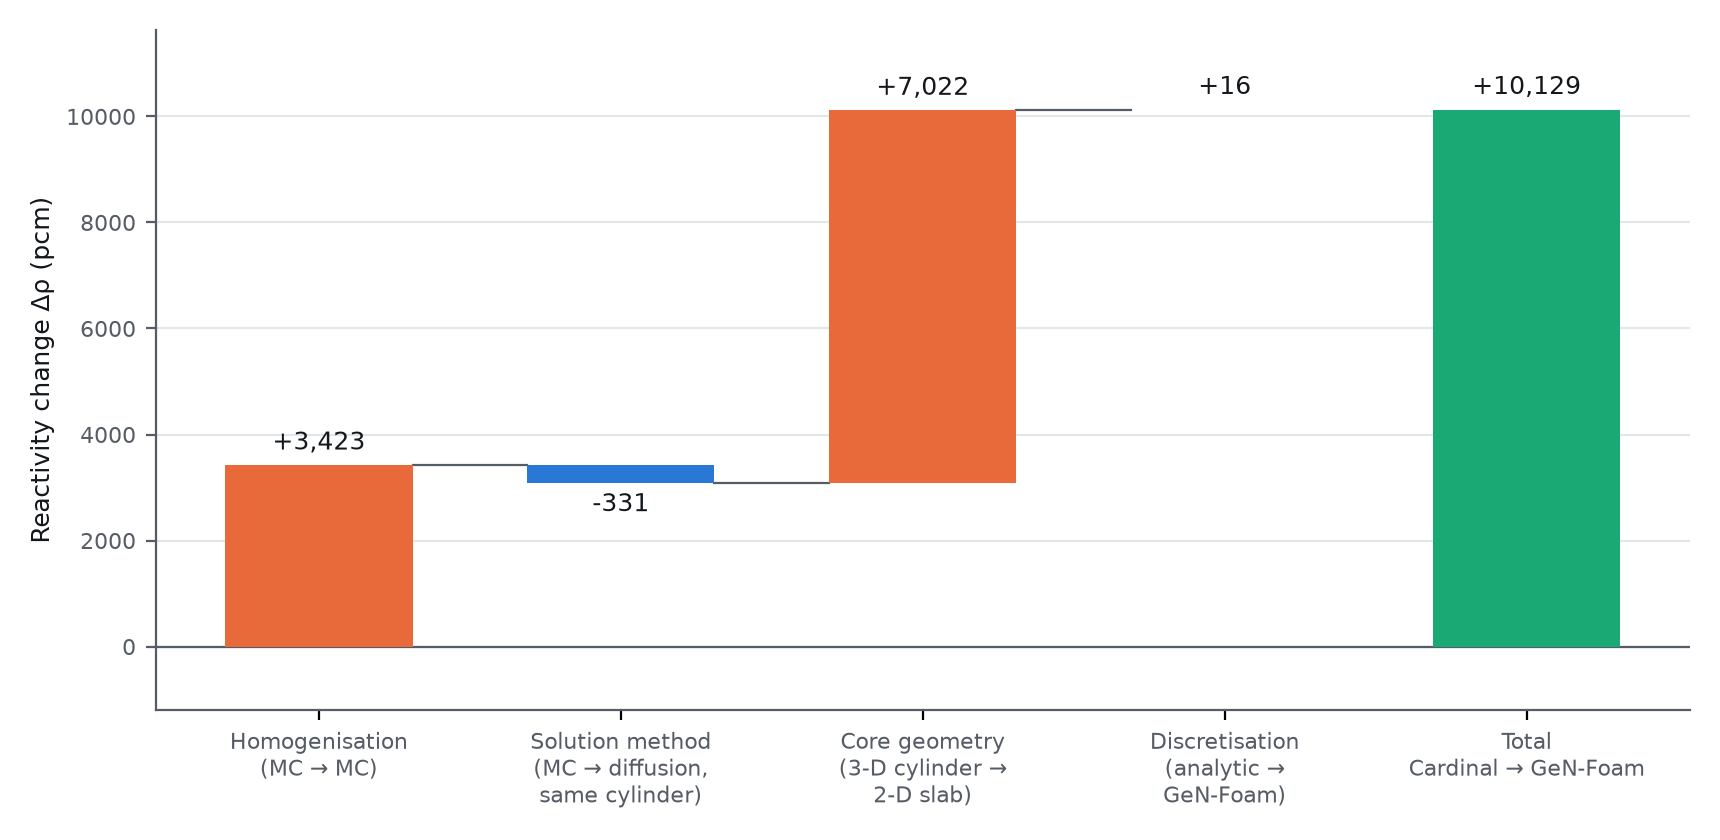
\includegraphics[width=.92\textwidth]{fig/fig6_keff.png}
\caption{Decomposition of the core eigenvalue difference into additive reactivity steps.}
\end{figure}

\begin{table}[H]\centering\small
\caption{Additive decomposition of the core eigenvalue difference.}
\begin{tabular}{@{}llrp{50mm}@{}}
\toprule
\textbf{Step} & \textbf{$k$: from $\rightarrow$ to} & \textbf{$\Delta\rho$} & \textbf{What it isolates}\\
\midrule
1. Homogenisation & $1.10206 \rightarrow 1.14526$ & $+3423$\pcm & Monte Carlo both sides; heterogeneous lattice $\rightarrow$ smeared zone\\
2. Solution method & $1.14526 \rightarrow 1.14093$ & $-331$\pcm & Same homogenised cylinder; Monte Carlo $\rightarrow$ 2-group diffusion\\
3. Core geometry & $1.14093 \rightarrow 1.24030$ & $+7022$\pcm & Same diffusion constants; 3-D cylinder $\rightarrow$ 2-D slab\\
4. Discretisation & $1.24030 \rightarrow 1.24054$ & $+16$\pcm & Analytic slab $\rightarrow$ GeN-Foam finite-volume solution\\
\midrule
\rowcolor{rowbg}
Total & $1.10206 \rightarrow 1.24054$ & $+10\,129$\pcm & Equal to the direct difference\\
\bottomrule
\end{tabular}
\end{table}

Three results follow.
\begin{enumerate}\itemsep2pt
\item \textbf{GeN-Foam's solver is verified.} Its numerical eigenvalue reproduces the analytic
two-group solution for its own geometry to 16\pcm{}.
\item \textbf{Geometry interpretation dominates.} Reading the core as a 2-D slab rather than a 3-D
cylinder accounts for about 70\% of the total difference.
\item \textbf{With geometry matched, diffusion and Monte Carlo agree closely.} In the same
cylinder, diffusion with GeN-Foam's constants and Cardinal's homogenised Monte Carlo differ by
$-331$\pcm{}, inside the 500\pcm{} criterion. With an extrapolated (Marshak) vacuum boundary
instead of zero flux the difference is $+1468$\pcm{}; both lie within the 1275\pcm{} spread of
the homogenised Monte Carlo result across hydrogen scattering kernels.
\end{enumerate}

The remaining $+3423$\pcm{} homogenisation step is the classical two-step error: smearing the
lattice removes resonance self-shielding and forces a single hydrogen thermal-scattering kernel
on a mixture whose hydrogen is 56\% ZrH-bound and 44\% water-bound.

\begin{callout}{Correction to an earlier version of this report}
An earlier version attributed $+8320$\pcm{} to diffusion-versus-Monte-Carlo method error,
assumed both cores were the same bare box, and treated \texttt{genfoam\_smoke\_keff} $=1.331$ as a
pin-cell method benchmark. Inspection of the GeN-Foam mesh showed the core is a 2-D slab, and
the smoke test was run on a separate channel geometry. The decomposition above replaces that
analysis.
\end{callout}

\subsection{Case 5 --- fuel temperature coefficient}
This is the most consequential physics quantity, because the coefficient governs the entire
transient response.

\begin{table}[H]\centering\small
\caption{Fuel temperature coefficient in GeN-Foam's operating band (500--\SI{600}{\kelvin}).
The comparison depends on which eigenvalue the coefficient is referred to.}
\begin{tabular}{@{}llr@{}}
\toprule
 & \textbf{Value} & \textbf{vs GeN-Foam}\\
\midrule
Cardinal, $\kinf$ --- unit cell, zero leakage & $-7.76$\,pcm/K & $-29\%$\\
\rowcolor{rowbg}
Cardinal, $\keff$ --- bare core, 20.1\% leakage & $\mathbf{-10.79\pm0.82}$\,\textbf{pcm/K} & $\mathbf{+7\%}$\\
GeN-Foam, transient (published constant) & $-10.000$\,pcm/K & ---\\
\bottomrule
\end{tabular}
\end{table}

A transient is driven by the \emph{core} eigenvalue, so the $\keff$-based coefficient is the
correct basis for comparison. On that basis the two values agree to \textbf{7\%}, within one
standard deviation of the Monte Carlo estimate. Because GeN-Foam's slab leaks less than the
specified cylinder, the coefficient appropriate to its own geometry would lie between the
lattice and cylinder values; the constant input is therefore, if anything, slightly too
negative for the slab. The apparent 29\% discrepancy against the
lattice value is an artifact of comparing an infinite-lattice quantity with a core quantity;
see Section~\ref{sec:leak}.

\begin{callout}{What remains open}
The magnitude of GeN-Foam's coefficient is \emph{corroborated} by the Cardinal core
calculation: $-10.0$ against $-10.79$\,pcm/K is agreement at the 7\% level, so the transient
results do not appear to be biased by the choice of coefficient.

Two points nevertheless remain. First, the coefficient is entered as a \textbf{constant},
whereas the computed value varies from $-6.3$ to $-10.8$\,pcm/K over
296--\SI{1000}{\kelvin}. A constant chosen to suit the 500--\SI{600}{\kelvin} band is too
negative below \SI{450}{\kelvin} and again above \SI{800}{\kelvin}, so a larger excursion
reaching higher fuel temperatures would be shut down more strongly than the physics supports.
Second, the input is a published value for a reflected TRIGA rather than one computed for
this bare-core model, so close agreement is partly fortuitous.

\textbf{Recommended action:} replace the constant with Cardinal's temperature-dependent
coefficient for transients leaving the 500--\SI{600}{\kelvin} band.
\end{callout}

\subsection{Cases 6--8 --- thermal quantities}
These cannot be differenced as reported, for three independent reasons:
\begin{enumerate}\itemsep2pt
\item \textbf{Cardinal describes an average pin.} Its own peaking factor of 2.2544 implies a hot
channel is materially hotter, so the two fuel temperatures do not describe the same object.
\item \textbf{Cardinal's film coefficient is a correlation, not a solution.} Dittus--Boelter at
$\mathrm{Re}=4755$ supplies 63\% of Cardinal's total temperature rise, and is applied outside its
reliable range.
\item \textbf{Cardinal's coolant CFD is a diagnostic only} (34.6\% energy closure, incomplete
heated-wall tagging), so no Cardinal coolant temperature is available for comparison.
\end{enumerate}

\subsection{Cases 10--12 --- no Cardinal counterpart}
The Cardinal model was scoped to steady state, so it has no transient counterpart. This is a
documented scope decision rather than an omission, but it means GeN-Foam's transient results
--- including the peak power on which the safety argument rests --- have \textbf{no independent
check}. Cardinal two-group constants were not generated either; GeN-Foam condensed its own
from OpenMC, and Case 4 shows these preserve the lattice eigenvalue to 33\pcm{}.

\newpage
%======================================================================
\section{Verification status}\label{sec:status}
\begin{callout}[alertbg]{This work is verified, not validated}
Verification asks whether the equations are solved correctly; validation asks whether the
equations describe reality, and is establishable only against experimental data.
\textbf{No experimental data was used in either calculation}, so no part of this study is
validated. Agreement between two codes is not a substitute --- two codes can agree and both
be wrong, particularly when they share a specification, a nuclear data library, or a
simplification. Here both share a bare-core model with no reflector and no control rods, so
\textbf{neither result describes a physical TRIGA at criticality}.
\end{callout}

\begin{table}[H]\centering\small
\caption{Verification status by level.}
\begin{tabular}{@{}llp{68mm}@{}}
\toprule
\textbf{Level} & \textbf{Status} & \textbf{Evidence}\\
\midrule
1. Software & MET & Both codes run to completion; GeN-Foam passes its reference cases; Cardinal conserves power exactly at \SI{2083.33}{\watt}\\
2. Numerical & PARTIAL & Cardinal neutronics converged (particles, seeds, Shannon entropy) and conduction converged; GeN-Foam matches the analytic two-group solution to 16\pcm{}; CFD is a diagnostic only; no mesh or order refinement study on either side\\
3. Physics & PARTIAL & Cardinal conduction within 1.1\% of analytic; ZrH feedback confirmed from nuclear data; GeN-Foam's feedback coefficient is a constant literature value, not computed for this model\\
4. Cross-code & PARTIAL & Lattice \kinf{} agrees to 280\pcm{}; core \keff{} difference fully decomposed, and agrees to 331\pcm{} once geometry is matched; fuel temperature coefficient agrees to 7\%\\
5. Experimental & NOT ATTEMPTED & No experimental data exists in this project\\
\bottomrule
\end{tabular}
\end{table}

\begin{table}[H]\centering\small
\caption{Actions required to close each gap, in priority order.}
\begin{tabular}{@{}rlp{58mm}l@{}}
\toprule
& \textbf{Gap} & \textbf{Action} & \textbf{Cost}\\
\midrule
1 & Core geometry differs & Re-run GeN-Foam on the specified 3-D cylinder & \SI{1}{\hour} CPU\\
2 & Constant feedback coefficient & Replace the literature constant with Cardinal's temperature-dependent coefficient; re-run the transient & \SI{1}{\hour} CPU\\
3 & CFD mesh tagging & Regenerate \texttt{fluid.re2} with the corrected generator; rerun NekRS & \SI{2}{\hour} GPU\\
4 & CFD not converged & Extend to $\sim$5 flow-throughs after resolving the filter undershoot & \SI{5}{\hour} GPU\\
5 & No mesh independence & Repeat at orders 5 and 8; compare integral quantities & \SI{8}{\hour} GPU\\
6 & Cardinal library deviation & Re-run coupled production on ENDF/B-VIII.0 & \SI{1}{\hour} CPU\\
7 & Reflector and rods & Add a graphite reflector and control rods to both models & ---\\
8 & No validation & Obtain TRIGA experimental data & ---\\
\bottomrule
\end{tabular}
\end{table}


\newpage
%======================================================================
\section{Limitations}
\begin{table}[H]\centering\small
\caption{Limitations of the present study, with their consequence for interpretation.}
\begin{tabular}{@{}p{48mm}p{88mm}@{}}
\toprule
\textbf{Limitation} & \textbf{Consequence}\\
\midrule
Both cores are bare & Neither model includes a reflector or control rods, so neither
describes a physical TRIGA at criticality. This is a \emph{shared} simplification, not a
difference between the calculations.\\
Core geometry differs & GeN-Foam models a 2-D slab, Cardinal a 3-D cylinder; the effect is
quantified ($+7022$\pcm) but the GeN-Foam core has not been re-run in the specified geometry.\\
Coolant CFD is a diagnostic & Incomplete heated-wall tagging, 34.6\% energy closure and a
filter undershoot below the inlet temperature; no CFD temperature is used.\\
Conduction uses a correlation & The Dittus--Boelter film coefficient supplies 63\% of the
Cardinal temperature rise and is applied at $\mathrm{Re}=4755$, outside its reliable range.\\
Average pin, not hot channel & Cardinal's peaking factor of 2.2544 implies a hot channel is
materially hotter than the reported temperatures.\\
Thermal properties assumed & $k_{\text{fuel}}$, $k_{\text{clad}}$, the film coefficient and
the coolant rise are documented modelling choices, not specification values.\\
Library deviation & The Cardinal coupled production run used ENDF/B-VII.1 rather than the
specified VIII.0; measured offset $+73$\pcm.\\
No mesh independence study & Neither side performed mesh or polynomial-order refinement.\\
Transient unverified & The transient was computed by one code only and has no independent
check.\\
\bottomrule
\end{tabular}
\end{table}

%======================================================================
\section{Reproduction}
Both calculations, all inputs and all result data are in the GitHub repository
\url{https://github.com/kavyawadhwa134/triga-crosscode-verification}.

\subsection{GeN-Foam}
\begin{table}[H]\centering\small
\begin{tabular}{@{}ll@{}}
\toprule
\textbf{Path} & \textbf{Contents}\\
\midrule
\texttt{genfoam/lattice/} & OpenMC pin cell and two-group MGXS extraction\\
\texttt{genfoam/tools/openmc2genfoam.py} & MGXS $\rightarrow$ GeN-Foam \texttt{nuclearData} converter\\
\texttt{genfoam/triga\_steady/} & Steady-state eigenvalue case (\texttt{Allrun}, \texttt{Allclean})\\
\texttt{genfoam/triga\_transient\_rod/} & $+0.5\,\$$ insertion transient (restarts from the steady case)\\
\bottomrule
\end{tabular}
\end{table}

\subsection{Cardinal / OpenMC / MOOSE / NekRS}
\begin{table}[H]\centering\small
\begin{tabular}{@{}ll@{}}
\toprule
\textbf{Step} & \textbf{Command}\\
\midrule
Environment audit & \texttt{./scripts/audit\_environment.sh}\\
Neutronics & \texttt{./scripts/run\_openmc.sh unitcell production --seed 11}\\
Coupled & \texttt{./scripts/run\_coupled.sh production 8}\\
Thermal-hydraulics & \texttt{./scripts/run\_nekrs.sh 8}\\
Temperature coefficient & \texttt{python cardinal/openmc/temperature\_coefficient.py}\\
Eigenvalue decomposition & \texttt{python results/comparison/keff\_decomposition.py}\\
\bottomrule
\end{tabular}
\end{table}

\begin{table}[H]\centering\small
\caption{Numerical settings for the Cardinal production runs.}
\begin{tabular}{@{}ll@{}}
\toprule
\textbf{Parameter} & \textbf{Value}\\
\midrule
Standalone neutronics & 40\,000 particles, 500 batches, 100 inactive ($2\times10^7$ histories)\\
Coupled neutronics & 20\,000 particles, 150 batches, 30 inactive, 10 Picard iterations\\
Solid mesh & 6400 elements, 20 axial layers\\
CFD mesh & 2880 spectral elements, polynomial order 7, 1\,474\,560 points\\
Coupled runtime & \SI{2905}{\second} wall, \SI{1132}{\mega\byte} peak\\
CFD runtime & \SI{4294}{\second} wall, \SI{2660}{\mega\byte} device, GTX 1080~Ti\\
\bottomrule
\end{tabular}
\end{table}

\subsection{Result files}
\begin{table}[H]\centering\small
\begin{tabular}{@{}ll@{}}
\toprule
\textbf{Path under \texttt{results/}} & \textbf{Contents}\\
\midrule
\texttt{genfoam/validation\_step\{2,5,6\}.csv} & GeN-Foam acceptance, lattice, core, transient\\
\texttt{genfoam/transient\_rod\_power.csv} & GeN-Foam transient time history\\
\texttt{cardinal/openmc\_unitcell.csv} & Cardinal \kinf, all configurations and seeds\\
\texttt{cardinal/openmc\_core*.csv} & Cardinal \keff, heterogeneous and homogenised\\
\texttt{cardinal/*temperature\_coefficient.csv} & Temperature-coefficient sweeps, lattice and core\\
\texttt{cardinal/coupled\_*.csv} & Coupled results per Picard iteration\\
\texttt{cardinal/thermal\_profiles.csv} & Axial and radial temperature profiles\\
\texttt{cardinal/nekrs\_convergence.csv} & CFD convergence history (diagnostic)\\
\texttt{comparison/crosscode\_comparison.csv} & Case-by-case comparison, machine-readable\\
\texttt{comparison/keff\_decomposition.csv} & Additive eigenvalue decomposition\\
\bottomrule
\end{tabular}
\end{table}

%======================================================================
\section{Conclusions}
\begin{enumerate}\itemsep4pt
\item \textbf{Where the two calculations solve the same problem, they agree.} The Monte Carlo
pin cell differs by 280\pcm{} at $3.1\sigma$, inside the 500\pcm{} acceptance criterion.

\item \textbf{The core eigenvalue difference is explained in full.} Of the $+10\,129$\pcm{}
difference, $+7022$\pcm{} comes from GeN-Foam modelling the core as a 2-D slab rather than the
3-D cylinder used by Cardinal, and $+3423$\pcm{} from homogenisation. With geometry matched,
two-group diffusion and Monte Carlo agree to 331\pcm{} (1468\pcm{} with an extrapolated
boundary), and GeN-Foam reproduces the analytic solution of its own geometry to 16\pcm{}.

\item \textbf{The ambiguous core dimension is the most important specification issue.}
``0.495 $\times$ 0.60\,m'' was read differently by the two models, and that reading is worth
about 7000\pcm{}. A benchmark specification should state the core shape explicitly.

\item \textbf{The fuel temperature coefficient is corroborated, with a caveat.} Cardinal
computes $-10.79\pm0.82$\,pcm/K for the bare core in the 500--\SI{600}{\kelvin} band from ZrH
scattering data, within 7\% of the published $-10.0$\,pcm/K constant used by GeN-Foam. The constant does not
capture the computed variation from $-6.3$ to $-10.8$\,pcm/K over 296--\SI{1000}{\kelvin}.

\item \textbf{Incomplete parts are reported as such.} The Cardinal coolant CFD is a diagnostic
only, and Cardinal did not attempt the transient. Neither is presented as a result.

\item \textbf{Neither calculation is validated.} Both cores are bare, without reflector or
control rods, and no experimental data was used. The study establishes cross-code
consistency --- not fidelity to a physical reactor.
\end{enumerate}

\vspace{5mm}\hrule\vspace{2mm}
\footnotesize\color{ink2}
Inputs, results and analysis scripts for both calculations:\\
\url{https://github.com/kavyawadhwa134/triga-crosscode-verification}.
Cardinal results were frozen at tag \texttt{pcm-independent-v1} before any GeN-Foam result was read.
\end{document}
